% !TeX root = ../main.tex
% Add the above to each chapter to make compiling the PDF easier in some editors.
\chapter{Farm Power Model}\label{chapter:power_model}

The first central component in optimizing the wind farm layout is to generate a data-driven surrogate Model that can be introduced into the optimization problem and solved by a solver. As detailed in the introduction, more specifically, the aim is to use the distCL extension to the Pyomo Python package, requiring a small Neural Network as a surrogate model. The following chapter documents the steps taken to generate such a model. To train such a Neural Network, data is required that covers the parameter space of the optimization to prevent extrapolation by the model. Therefore, the chapter starts by explaining how the open-source wind farm simulation tool FLORIS® was used to generate a dataset and what the simulations behind this dataset are. Then, the fundamentals of Neural Network architecture and training are briefly introduced, before the model of the interactions for two turbines is trained and evaluated.



\section{Data Source}

The power output of wind turbines and wind farms as a whole is fundamentally connected to the aerodynamic conditions in the airflow every wind turbine experiences, with wind speed as the biggest factor relevant to how much power a wind turbine can generate. The main effect reducing the power generated by a wind turbine is to be positioned in the wake downwind of another turbine. This power reduction is primarily a result of the reduction in windspeed joined with the increased turbulence in the wake airflow (see \ref{fig:wake_photo})  \cite{KIRANOUDIS1997439}. Moving further downstream of a wind turbine, the wake gradually mixes with the outer airflow and thus again increases windspeed until the entire airflow reaches a new homogeneous air speed \cite{MAGNUSSON1999169}. Thus, even if a wind turbine is positioned in the wake of another wind turbine, the greater the distance between the two, the less the second wind turbine is affected. Ideally, wind turbines are not positioned in the wake of other wind turbines at all. 

\begin{figure}[h] 
	\centering
	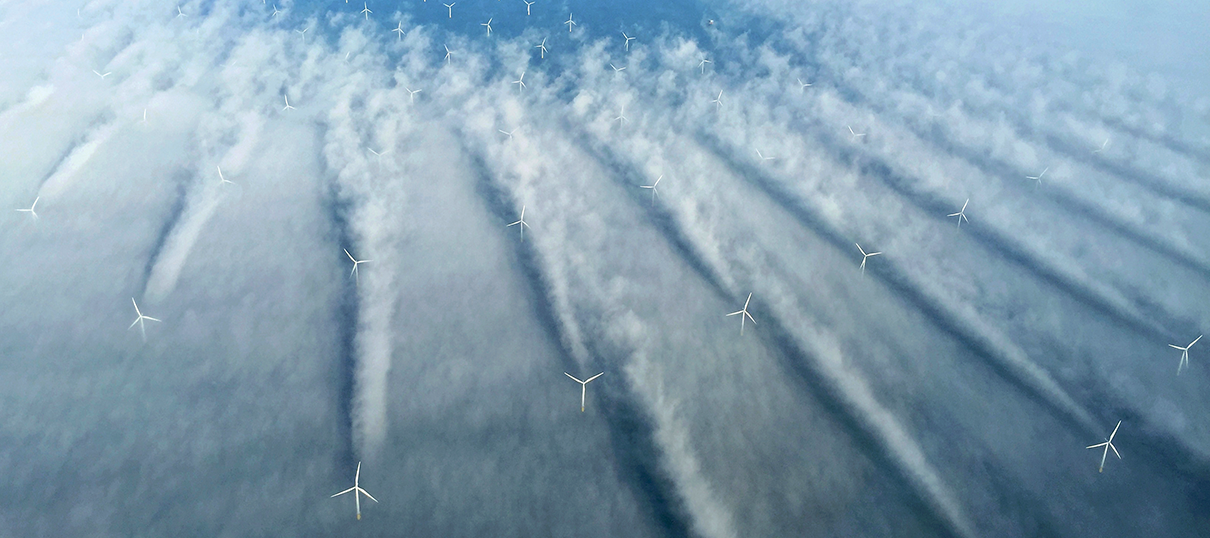
\includegraphics[width=0.8\textwidth]{figures/introduction/wake_photo.png} 
	\caption{Visible wind turbine wakes due to contrail generation \cite{windpowermonthly_offshore_clusters}}
	\label{fig:wake_photo}
\end{figure}


With the overall goal of creating a model that models how the interaction between wind turbines (induced by the wake) is related to the wind turbines relative positioning to each other and the wind conditions as input to an optimization model, a tailor-made dataset from simulation results is the easiest to handle to ensure that the data fits the use case well. Using self-generated simulation data allows to set the parameter space of the model as required for the different variants of the optimization problems explored in the second part of this thesis. After investigating two Python-based open source wind farm simulation tools FLORIS (\href{https://www.nrel.gov/wind/floris}{FLORIS official website}) and PyWake (\href{https://topfarm.pages.windenergy.dtu.dk/PyWake/}{PyWake Documentation}), FLORIS was chosen after a brief comparison between the two due to its apparent ease of use. The FLORIS is a wind farm simulation tool developed by the National Renewable Energy Laboratory (NREL) as one of multiple tools containing models of varying complexity available for different use cases. FLORIS is a control-systems-oriented toolbox and therefore contains a lower complexity model yielding fast simulation results. This allows the automatic generation of large quantities of data in a relatively short time. As the data is coming from  simulation results, the data is deterministic even though there is an underlying uncertainty attributed which can be quantified by FLORIS if required. 

For this thesis, depending on the optimization problem, FLORIS is given a grid of the following parameters:

\begin{itemize}
	\item Position of Wind Turbines
	\item Wind Direction
	\item Wind Speed
	\item Wind turbulence
\end{itemize}

 defining the parameter space limits with evenly spaced data points to then generate the corresponding simulation data, with the simulation outputs being the generated power by the individual wind turbines as well as by the farm as a whole (e.g. the sum of individual power outputs). The configuration of all of these parameters, as well as the number of wind turbines, can be modified at will in this setup and the result is a dataset with the rows corresponding to a specific combination of parameters and the resulting power outputs of the turbines. As a turbine type, an IEA 10-MW is used for data generation due to its repeated use as a baseline turbine in other scientific works like \cite{Madsen2022} and \cite{Kainz2024IEA}, a more exact technical specification of the turbine can be found in \cite{Bortolotti2019}. The configurations of the specific dataset generated for the individual optimization problem formulations are documented in the corresponding Sections of Chapter \ref{section:optimization}.


\section{Introduction to Neural Networks} \label{sec:modelling}

To model the relationship between the attributes of an incoming airflow to a wind turbine and the output generated by the same wind turbine, many surrogate models could be chosen. As the model generated for this thesis is created to be then introduced into the Pyomo extension referenced in Chapter \ref{chapter:introduction}, the model has to be compatible with said extension. That is why the model chosen is a simple neural network with a limited number of hidden layers and nodes, with the size of the Neural Network being limited due to its introduction into the optimization problem. 

In the following section, a brief introduction is given to how Neural Networks work and are trained, including some regularization techniques.

\subsubsection{Architecture of a Neural Network}

Fundamentally, Neural Networks represent Graph Networks consisting of function blocks as the nodes, in the case of Neural Networks called perceptrons (or Neurons as a more general term) and arcs which correspond to the inputs/outputs of a given perceptron. In simple words, the inputs to the Neurons are summed up and introduced as an argument into a function $f()$, which yields an output $y$, representing the output of the given perceptron. These Neurons are organized in layers, which correspond to the row-type structure Neural Networks are usually represented in and each perceptron of one layer is connected to every other perceptron of the following layer. The following layer, in this case, means in the direction of flow, in visualizations usually from left to right. The arcs thus in simple terms correspond to a single number, and the Neurons to the action of summing up all inputs and then applying the unspecified function $f()$ to generate an output. This process is repeated for all Neurons in the network, with the first layer of the network taking as input the values of the given data features (the input values to the model) and the last layer producing outputs corresponding to the output value(s) of the model. The number of Neurons in this first and last layer corresponds to the task the Neural Network is supposed to perform. If the goal is to identify handwritten numbers 1-9 from 50x50 pixel images, the input layer might have 50x50 Neurons for the value of each pixel, and the output layer 9 layers with the output value of each perceptron representing how much the network "thinks" the given image shows the corresponding numbers 1-9. A schematic of this architecture is given in Figure \ref{fig:neural_network_architecture}.

\begin{figure}[h] 
\centering
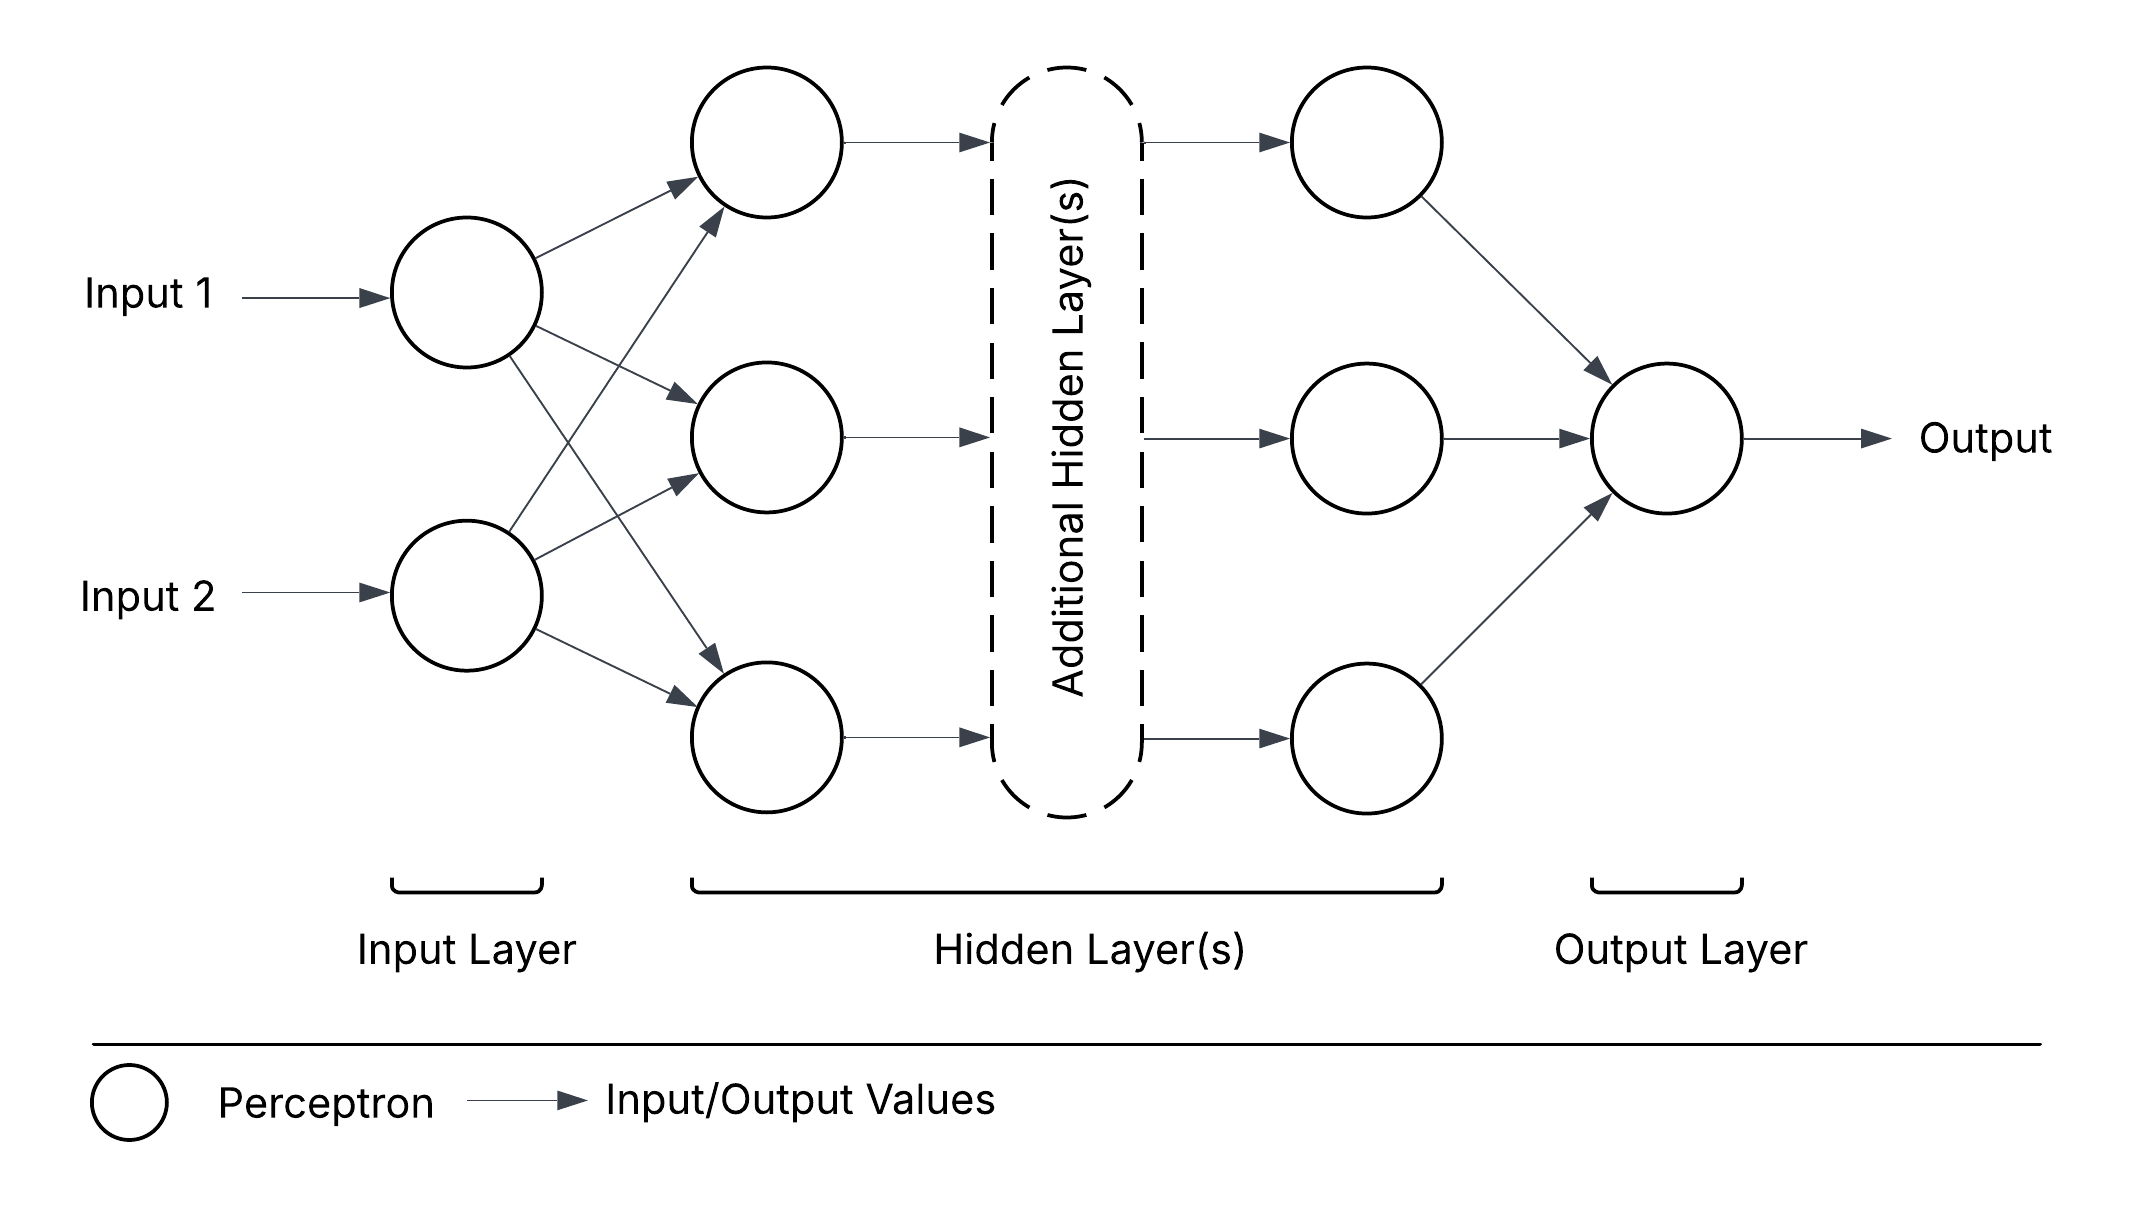
\includegraphics[width=0.9\textwidth]{figures/modelling/neural_network_concept.png} % file name without extension
\caption{Schematic of Neural Network Architecture}
\label{fig:neural_network_architecture}
\end{figure}

As shown in Figure \ref{fig:neuron_calculations} the output of a Neuron is slightly more complicated as described before, as the output $y$ is generated by summing up the inputs $x$ multiplied by a corresponding weight $w$ together with a bias $b$ and introducing this summation as an argument into an activation function $f()$. In this process, the weights $w$ represent a weight to give importance to the individual inputs and the bias $b$ serves to set a minimum output value that will always be reached, regardless of the inputs. 

\begin{figure}[h] 
	\centering
	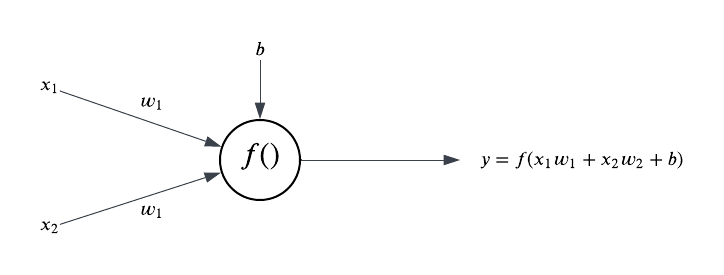
\includegraphics[width=0.8\textwidth]{figures/modelling/perceptron_concept.png} % file name without extension
	\caption{The output of a neuron is generated by applying the activation function to the sum as the weighted inputs $w_ix_i$ and the bias of the neuron $b$}
	\label{fig:neuron_calculations}
\end{figure}

The activation function $f()$ is called the activation function, as in its simplest form it represents a step function that decides if a neuron activates or not, e.g., takes the binary values ${0,1}$ for a given threshold. Contrary to the human brain, where neurons are indeed binary, most Neural Networks resort to an activation function whose outputs are not binary but deliver continuous values between $0$ and $1$ to avoid the boundary issues that occur with binary thresholds. The most common function used instead of a step function is the sigmoid function, which roughly corresponds to a continuous version of the step function, with $\sigma(x) \approx 1$ for $x \to \infty$ and $\sigma(x) \approx 0$ for $x \to -\infty$.


\[
\sigma(x) = \frac{1}{1 + e^{-x}}
\]

This relationship also becomes apparent when plotting both of those functions over each other, as shown in Figure \ref{fig:activation_functions}. 
An alternative to the sigmoid as activation function is the Rectified Linear Unit (ReLu) function, or in simple words, the maximum function, defined as follows. 

\[
\text{ReLU}(x) = \max(0, x) = 
\begin{cases}
	0 & \text{if } x < 0, \\
	x & \text{if } x \geq 0.
\end{cases}
\]
 
 The main general applicable benefit of the ReLu function is that it has a constant, non-vanishing gradient for both directions (see Figure \ref{fig:activation_functions}), leading to better gradient propagation, an attribute that is relevant in the context of the backpropagation algorithm briefly discussed in Section \ref{subsubsec:training_nn}. \cite{preprintReLuGlorot}
 Beyond this, the ReLu function allows for embedding the Neural Network into a conventional optimization problem, as will be discussed in Section \ref{sec:constraint_learning}.

\begin{figure}[h] 
	\centering
	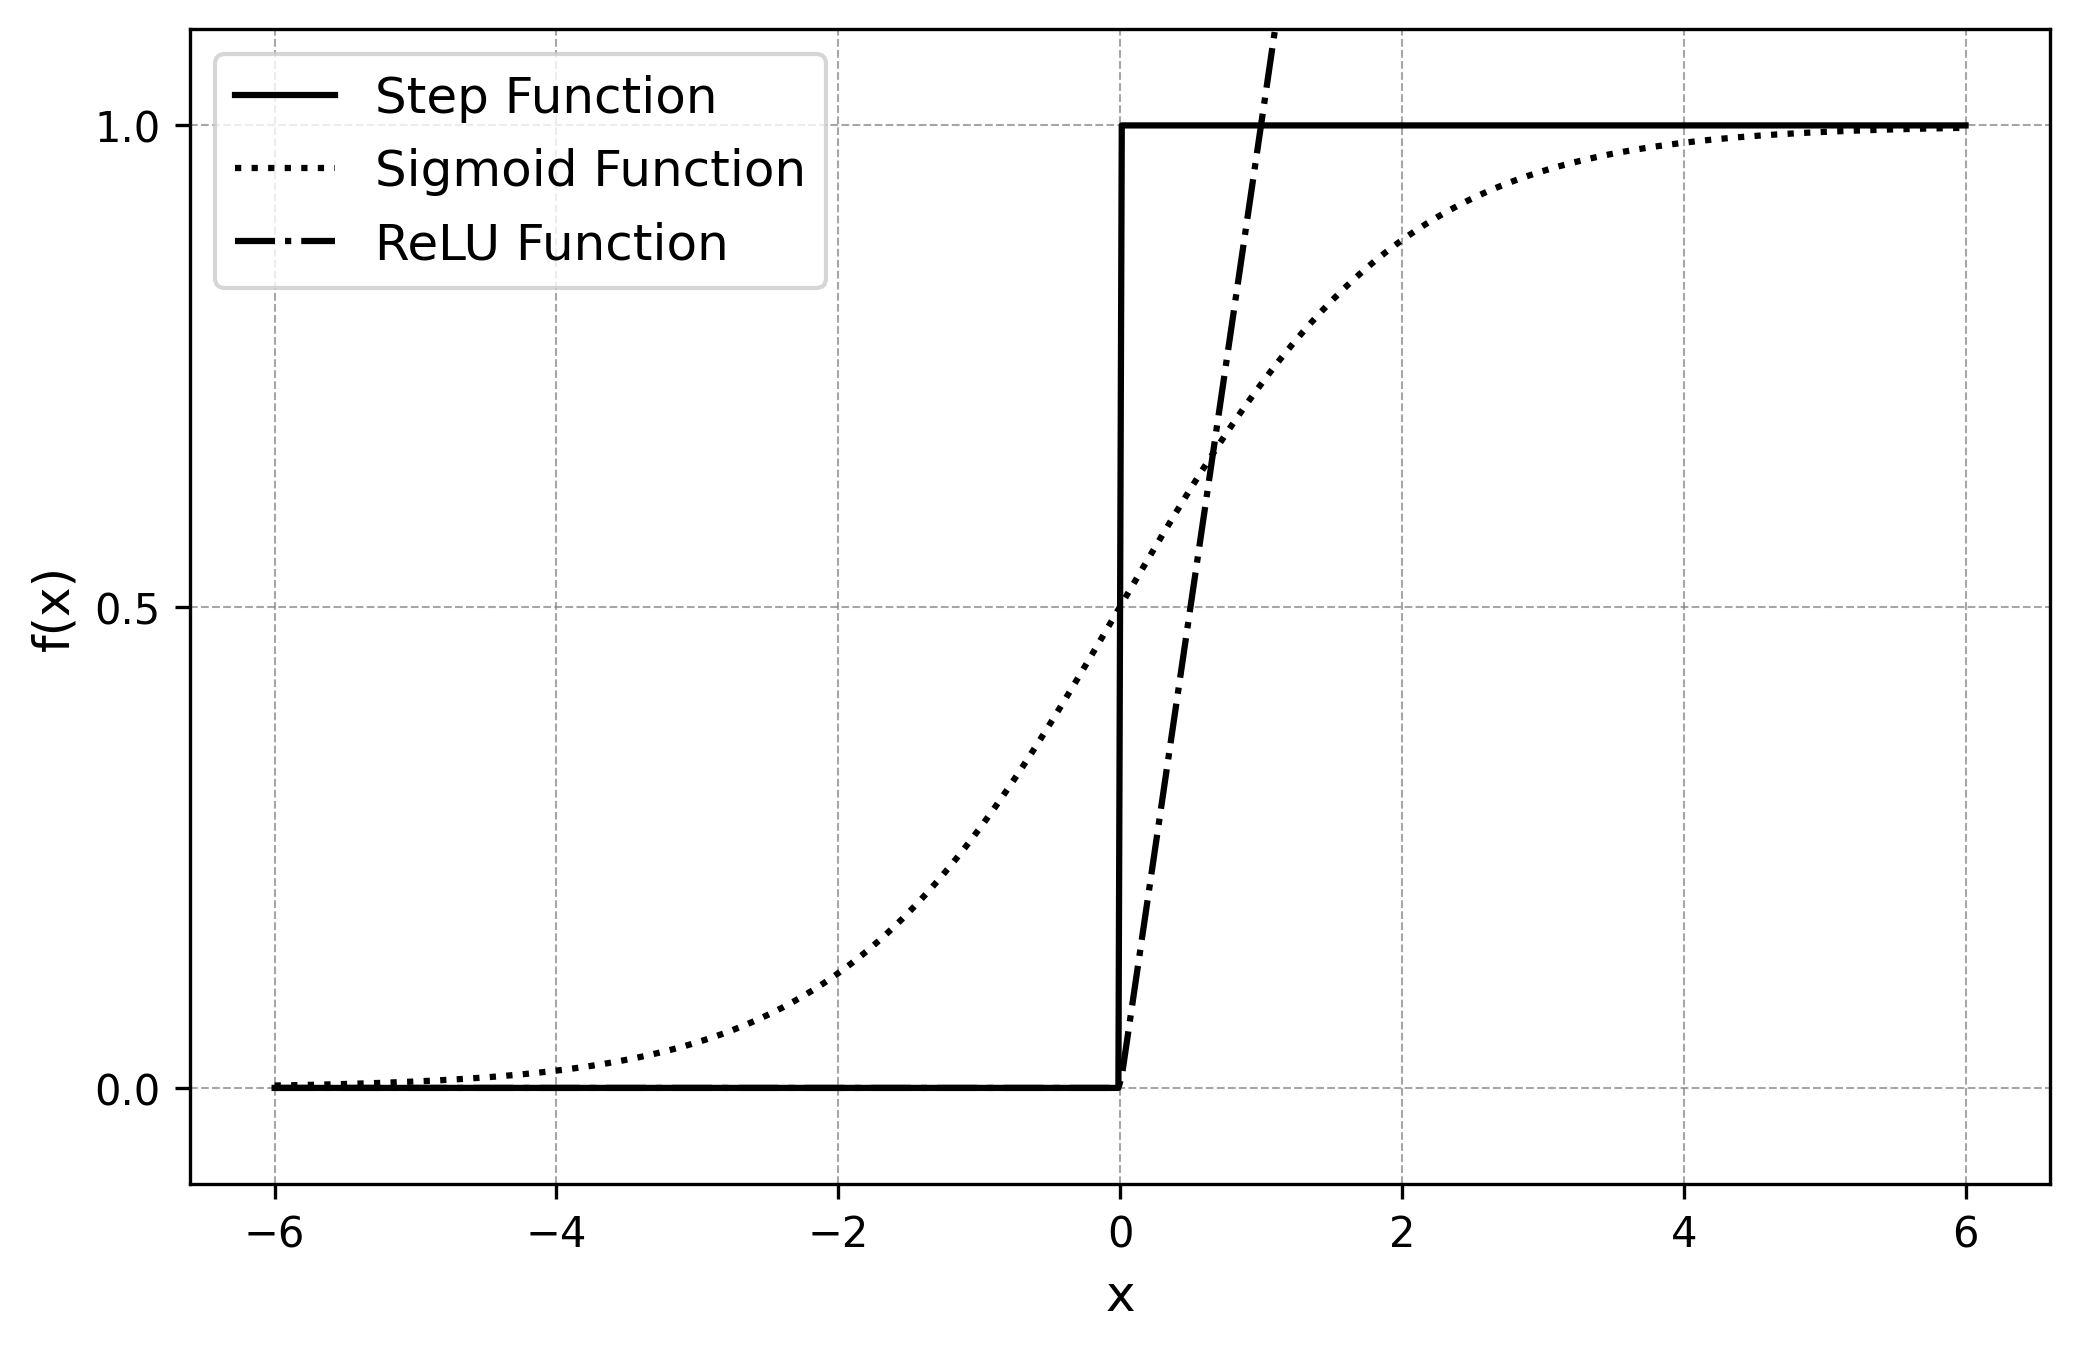
\includegraphics[width=0.9\textwidth]{figures/modelling/activation_functions.png} % file name without extension
	\caption{The Sigmoid Function being close to the Step Function without being as sensitive to slight changes in $x$ due to its continuity. Alternatively, the Rectified Linear Unit function (ReLu) can be used as activation function. }
	\label{fig:activation_functions}
\end{figure}

\cite{nielsen2015neuralChap1}


\subsubsection{Training a Neural Network} \label{subsubsec:training_nn}

With the general structure set up, and assuming that a layout has been chosen for the neural network (e.g. number of layers and number of their corresponding neurons), the training of the neural network corresponds to adjusting the weights $w$ and the biases $b$ of each neuron in a way, that allows the model to perform the task it is given well. What it means for the model to perform well is defined by a \textit{Loss Function}, which defines a relationship between the output of the model and the correct output (defined by training data) and gives a Loss as output, which is some sort of delta between model prediction and truth. What it means for a model to perform well heavily depends on the task (regression, binary classification, multiclass classification, etc.), but regardless of the task, the goal is always to minimize the Loss Function. A well-known Loss Function in regression is the Mean Squared Error (MSE)

\[
\text{MSE} = \frac{1}{n} \sum_{i=1}^{n} (y_i - \hat{y}_i)^2
\]

The training of the Neural Network thus corresponds to adjusting the weights and biases in a way that minimizes the chosen loss function. The algorithm most commonly used for this is called \textit{Backpropagation}.
 \cite{nielsen2015neuralChap1}
 
 Before diving into how the algorithms work exactly, it makes sense to first define specifically what parameters have to be optimized, e.g., all weights and biases of the network to be optimized. A common notation of the individual weights is as $w_{jk}^l$ with $l$ being the layer of nodes into which $w_{jk}^l$ are the weights of its inputs ( weighing the values from the outputs of the $(l-1)^{th}$ layer) and $j$ as the neuron from the $l^{th}$ layer as well as $k$ the neuron of the  $(l-1)^{th}$. Similarly, the biases are written as $b_j^l$ with $l$ as the layer and $j$ the neuron in that layer as as can be seen for both the weights and bias in an example in Figure \ref{fig:bias_and_weights_notation}.
 
 
 \begin{figure}[h] 
 	\centering
 	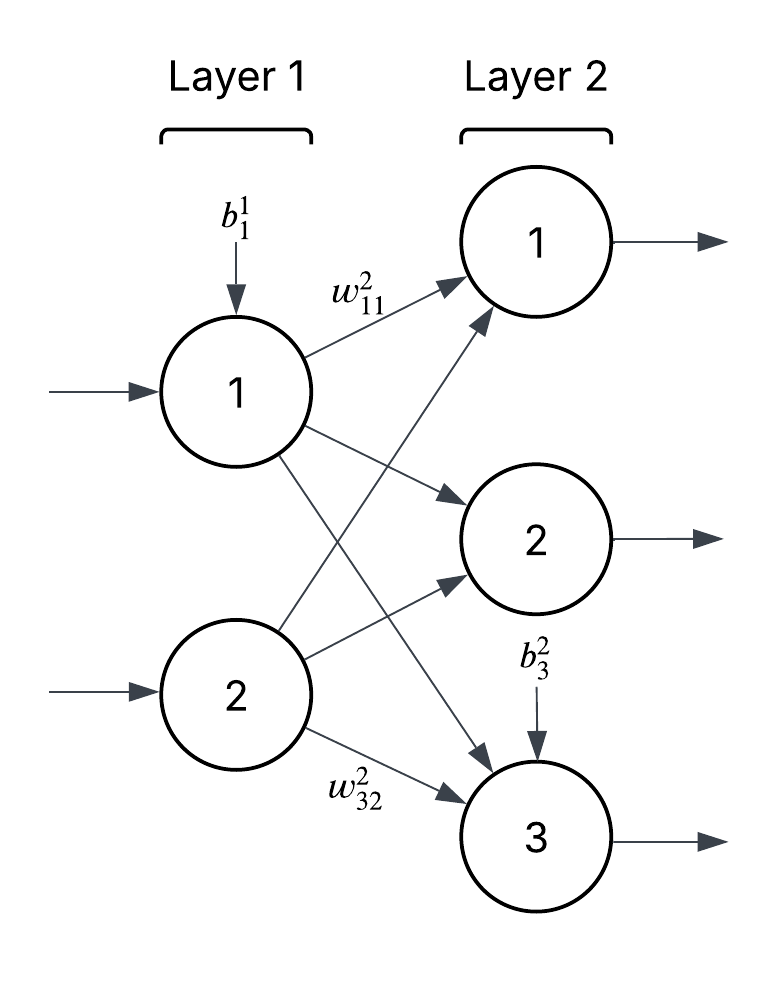
\includegraphics[width=0.4\textwidth]{figures/modelling/bias_and_weights_notation.png} 
 	\caption{Notation of Neural Network weights and biases with weight $w_{jk}^l$ and $l$ being the input layer,  $j$ the neuron from that input layer and $k$ the neuron of the  $(l-1)^{th}$ output layer. Similarly, the bias as $b_j^l$ with $l$ as the layer and $j$ the neuron.}
 	\label{fig:bias_and_weights_notation}
 \end{figure}
 
 Using this notation, the output of a given neuron $a_j^l$ can be calculated as 
 
 $$
 a_j^l = \sigma\left( \sum_k w_{jk}^l a_k^{l-1} + b_j^l \right),
 $$
 
 This expression can be further simplified by writing weights and biases in matrix form, using for each layer, a weight matrix $w^l$ for all weights input into the given layer $l$ and a bias vector $b^l$. By doing so, the output vector $a^l$ of the entire layer $l$ can be calculated as.
 
 $$a^l = \sigma (w^la^{l-1}+b^l)$$
 
With the notation for weights and biases established, the goal becomes tuning them in such a way as to minimize a chosen Loss function as discussed above. This is done by using training data with a known correct output and changing weights and Biases in such a way that moves the Neural Network towards outputting the true known value. 
The algorithm to do so essentially corresponds to: 

\begin{enumerate}
	\item Introduce Training Data into the Neural Network
	\item Evaluate the Loss Function for the Training Points (with small random values for weights and biases for the first iteration) and evaluate the gradients of the Loss function for the gradients of the individual weights and biases ($\frac{\Delta Loss}{\Delta w_{jk}^l}$, $\frac{\Delta Loss}{\Delta b_j^l}$) using backpropagation  \footnote{The Gradient can either be evaluated for each training point individually or for batches of training points}
	\item Update the weights and biases according to a learning rate $\rho$ weighted by the specific weight or biases gradient like $w_{jk}^l =w_{jk}^l - \rho \frac{\delta Loss}{\Delta w_{jk}^l}$ and $b_j^l =b_j^l - \rho \frac{\Delta Loss}{\Delta b_j^l}$ 
	\item Repeat process $n$ Epochs, with one Epoch being the algorithm passing through all training points/batches of points once
\end{enumerate}

This algorithm represents a gradient descent algorithm with learning rate  $\rho$ corresponding to the step length while evaluating the partial derivatives $\frac{\Delta Loss}{\Delta w_{jk}^l}$, $\frac{\Delta Loss}{\Delta b_j^l}$ is the critical step. Here, the backpropagation algorithm gives an efficient method of finding these partial derivatives by evaluating the individual error contributions of each Neuron and how errors accumulate as the inputs move through the Network. A more extensive explanation of how backpropagation works can be found in \cite{nielsen2015neuralChap2}. As is common for gradient descent, finding the global optimum for the weights and biases is not guaranteed and is even improbable if many local minima exist, as they do for the many parameters of a Neural Network. Nonetheless, using gradient descent, it is hoped to find a good local minimum. \cite{James2023} \cite{nielsen2015neuralChap2}

 \subsubsection{Regularization}
 
 Like most machine learning models, Neural Networks run at risk of overfitting. Neural Networks are especially prone to overfitting due to their many degrees of freedom represented by the many biases and weights, potentially exceeding the number of training samples.

 To prevent overfitting, regularization techniques like Cross-Validation can be applied in training, as for any other model. One very specific regularization method for Neural Networks is \textit{Dropout Learning}, which corresponds to randomly removing Neurons from the network (by effectively setting their activation function and thus their output to 0) for each training observation. By other nodes having to "stand in" for the dropped-out nodes, nodes are prevented from developing overspecialization. \cite{James2023}



\textbf{Notes}
- many Degrees of Freedom, many local maxima
- Adaptive Moment Estimation (ADAM) optimization

\subsubsection{Estimating Distributions using Neural Networks }

Neural Networks can also be used to estimate distributions of a random variable. Two possible approaches are to so-called Quantile Neural Networks and Distributional Neural Networks. While their Architecture is that of a normal Neural Network as discussed in the previous section, they differentiate in the output layer, where the Quantile Neural Network has outputs that correspond to the probability for a specific quantile while the distributional Neural Network outputs the distribution, like in Figure  \ref{fig:quantile_dist_nn} for a normal distribution.


\begin{figure}[h] 
	\centering
	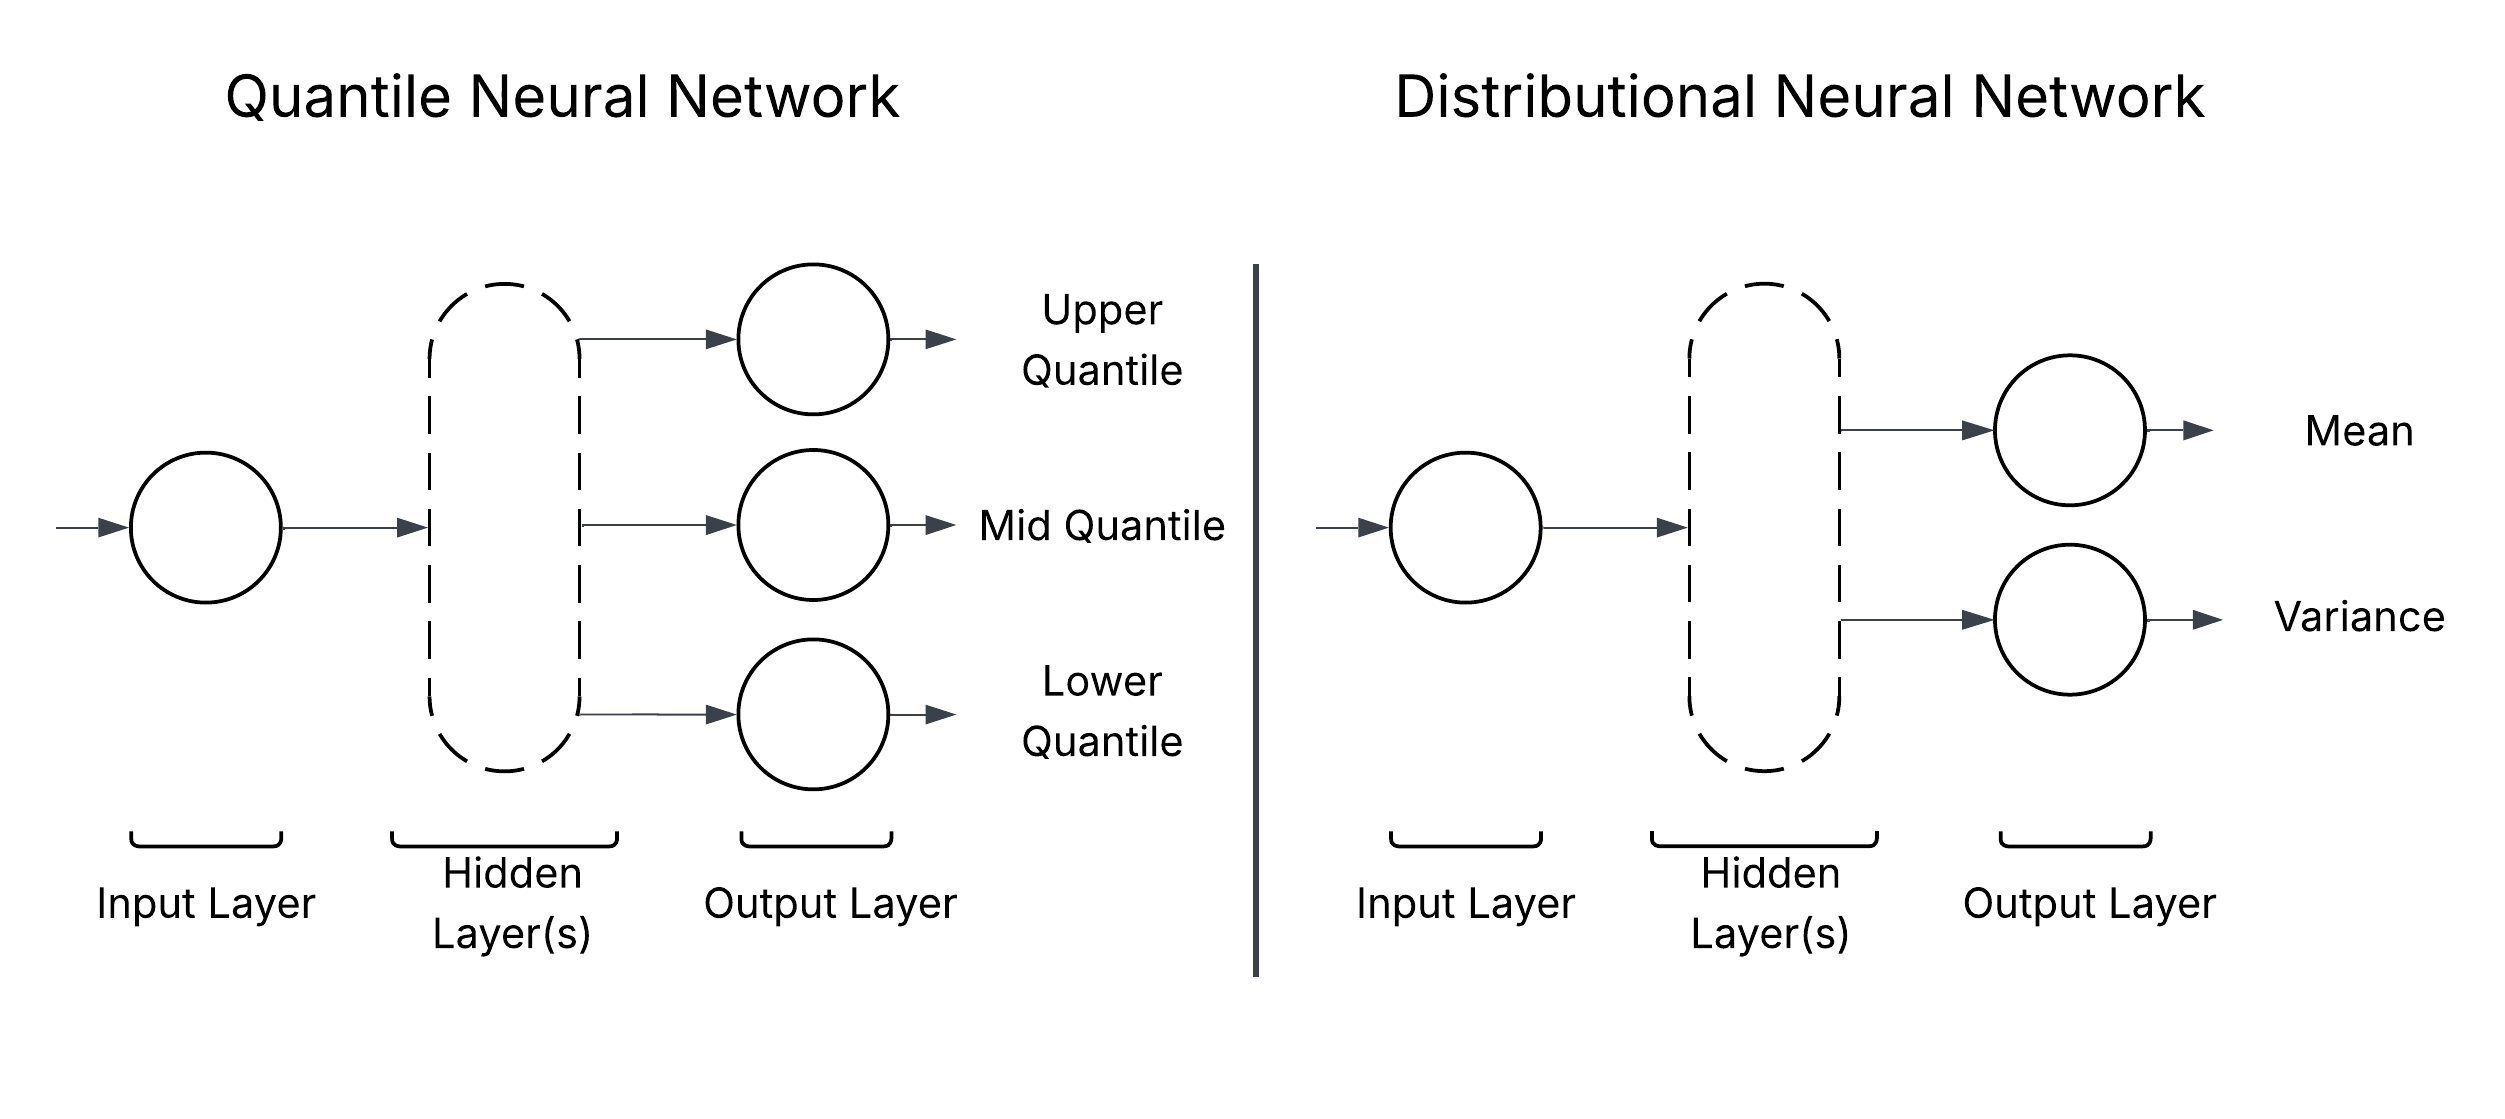
\includegraphics[width=0.9\textwidth]{figures/modelling/quantile_dist_nn.png} 
	\caption{Neural Networks to estimate a distribution by estimating specific quantiles (left) or the parameters of a distribution (right)}
	\label{fig:quantile_dist_nn}
\end{figure}

The different outputs from both neural Networks require appropriate Loss functions. For Quantile Neural Networks, the Pinball Loss (Quantile loss, for more see \cite{Steinwart_2011}) is used, while in the case of Distributional Neural Networks, the Likelihood (like in the form of the Negative Log Likelihood)  can be used as commonly used in classical statistics for parameter estimation. 

\cite{Akpabio} \cite{Marcjasz_2023}

\section{Modelling Pipeline} \label{sec:model_pipe}

With the theoretical foundations laid out, this section is going to treat the actual training process of the Neural Networks to be introduced into the optimization. Part of the challenge of training Neural Networks for this specific purpose is that the objective in optimizing the Neural Network is not only to minimize the cost function, but also to minimize the  number of model parameters, e.g., to minimize the total number of neurons the network consists of. This is because each neuron corresponds to an additional three linear constraints in the optimization problem, leading the number of constraints to grow as $\Delta n_{constraints} =3 \times \Delta n_{neurons}$. In general, individual models are trained for each optimization problem seen in Chapter \ref{section:optimization} tailored to their individual needs and parameter space. This is why this chapter will detail the main components of the modeling process and parameters that will be defined according to the optimization problem later on. The exact configuration of the models will then be defined together with the optimization problem.  

The modelling pipeline contains three main components, with the elements consisting of the data generation, hyperparameter tuning (training), and the final model training as seen in in Figure \ref{fig:model_flow}, where data generation corresponds to running the required simulations via FLORIS  for the given parameter space, hyperparameter tuning corresponds to the training and evaluation of different model configurations and final model training as the step in which the final model that is to be introduced into the optimization problem is trained.


\begin{figure}[h] 
	\centering
	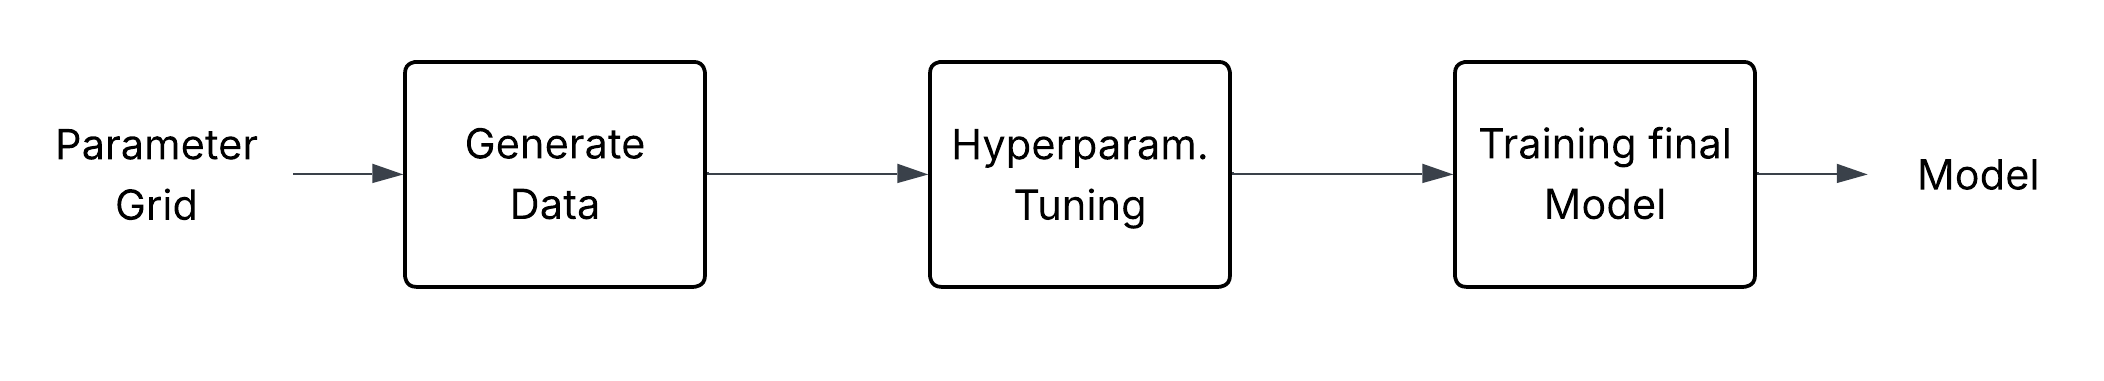
\includegraphics[width=0.9\textwidth]{figures/modelling/model_flow.png} 
	\caption{Flow of model generation, with parameter grid as input and the final model as output}
	\label{fig:model_flow}
\end{figure}

\subsubsection{Data Generation}

The Data Generation corresponds to the creation of a dataset corresponding to a grid that is set up within the parameter space of the optimization problem. The objective is to generate a dataset that covers the parameter space with sufficient density to train a model that is able to accurately interpolate between the given data points. Each  data point corresponds to an individual simulation performed using the tool FLORIS, allowing for an array of inputs and delivering an array of outputs. As inputs, the following variables can be defined as part of the parameter grid:

\begin{itemize}
	\item x\_range
	\item y\_range
	\item wind\_speeds
	\item wind\_directions
	\item turbulence\_intensities
\end{itemize}

Where x\_range and y\_range correspond to the relative distances of the second wind turbine to the first, wind speed corresponds to wind velocity in m/s,  direction to the incoming wind angle in Degrees (with 0° corresponding to norht, 180° to south) and turbolence intensities as a measure of turbolence for the incoming airflow. Figure \ref{fig:Floris} shows an example of a simulation output. 


\begin{figure}[h] 
	\centering
	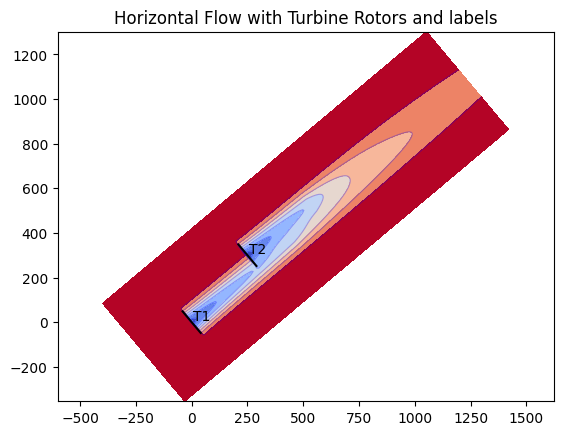
\includegraphics[width=0.7\textwidth]{figures/modelling/Floris.png} 
	\caption{Example of a Simulation output from the FOLORIS Wind Turbine Simulation Tool with colormap corresponding to airflow velocity}
	\label{fig:Floris}
\end{figure}

The method implemented in [LINK TO GITHUB https://github.com/schmeti/uc3m_TFM_wind_farm_optimization_codebase/blob/main/Windfarm_power_modelling/src/simulate_data.py] takes a range of values together with a specified number of chosen steps for the specific parameter and performs a simulation for all combinations for the given ranges to fill the entire grid. As the number of steps or limits may be different for the different parameters, the grid is not necessarily equally spaced for all parameters, but for each parameter individually is constant, e.g. the distance between values is the same for the entire range.  
Depending on the configuration of the problem, some parameters may be constant. If, for example, a variable like turbulence intensity is not taken into account for a given optimization, a constant value is set, and the data is generated for that constant value. The model trained on this dataset is thus constrained in use to the assumption of that specific constant, a limitation that is important to keep in mind further down the road when the initial dataset generation might not be as conscious anymore. 

The outputs of the simulation are:
\begin{itemize}
	\item Total Power Generation
	\item Power generated by Turbine 1
	\item Power generated by Turbine 2
\end{itemize}

where the total power generation corresponds to the summation of the power generated by the individual turbines. To maximize total farm output, the total power generation will now be used as a target for the model in the following steps.

\subsubsection{Neural Network Configuration}

The next step in the process corresponds to the hyperparameter tuning of the Neural Network. According to the chosen type of Neural Network (distributional Neural Network or single output Neural Network), an appropriate loss function has to be chosen first. The data is then split into a training and an evaluation set, and the model is trained on the training partition using the algorithms detailed in  \ref{subsubsec:training_nn}, using backpropagation/gradient descent as well as dropout learning for regularization for a chosen number of times.  

Once the training process is ended, the model is used to predict for the test partition of the data, and the results are evaluated by scoring the predictions using the Mean Squared Error (MSE). 

This process is repeated for a grid of the hyperparameters:
\begin{itemize}
	\item Number of Hidden Layers
	\item Number of Nodes in each hidden layer
\end{itemize}

and a plot like shown in Figure	\ref{fig:hyperparm} generated to decide what the best configuration of the Neural Network is. 

\begin{figure}[h] 
	\centering
	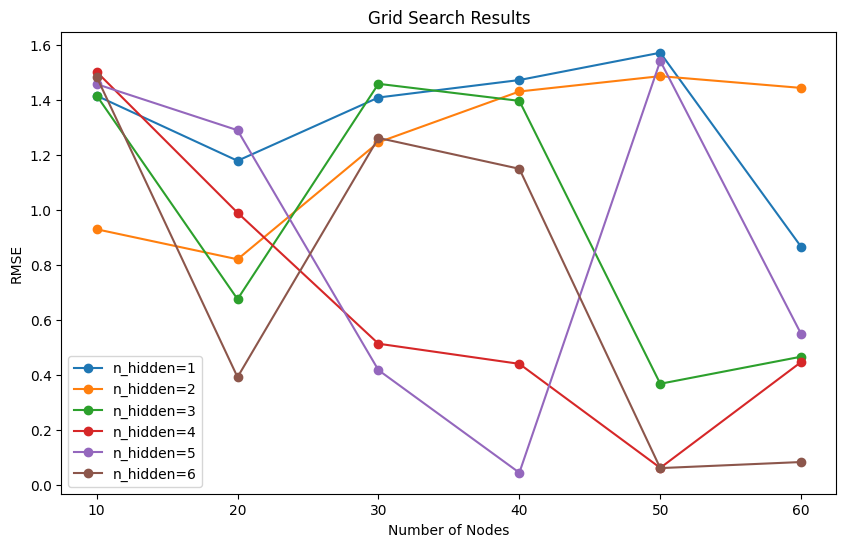
\includegraphics[width=0.8\textwidth]{figures/modelling/hyperparm.png} 
	\caption{Exemplary Output of Hyperparameter tuning with number of hiden layers $n_{hidden} $ and number of nodes per hidden layer}
	\label{fig:hyperparm}
\end{figure}

The final decision on what is the ideal model configuration is not only based on the best performance, but via the trade-off between complexity and output, to generate a model that is as small as possible. The kind of optimization problem the model will be used to solve is further taken into account, with complex optimization problems having less tolerance for a complex model.


\subsubsection{Final Model Training}

After having chosen a specific model configuration, a model is then trained using that configuration. This is the model that is eventually introduced into the optimization problems detailed in Chapter \ref{section:optimization}.

\section{Possible Improvements in the Modelling Process}

As one of the two main components of the optimization process, the model generation step shows some potential for improvement in the future. The currently evenly spaced grid of data points could be replaced by a grid that is organically generated according to the gradient of the underlying function by providing a denser grid in areas of large changes in the power function to provide the Neural Network with more data in these areas. The result could be an improved accuracy and efficiency, with data points concentrated on areas of interest.   

To reduce the size of the Network, the number of Neurons could be allowed to change from hidden layer to hidden layer and allow for removing expendable Neurons. 

To improve the accuracy of the models, a higher-quality simulation method could be used to generate the dataset. While this might come at a computational cost, the more accurate data might lead to an increase in the  accuracy of power output prediction, which, depending on the application context, might be worthwhile.  

Beyond these two proposals, it is safe to assume that a wide range of methods are available to improve performance and efficiency. These might be worthwhile to pursue once the method developed in this thesis has been shown to provide a valuable new approach to wind turbine positioning optimization.
